\documentclass[11pt,twocolumn]{article}

% ============================================================
% Packages
% ============================================================
\usepackage{shared/luxcover}
\usepackage[utf8]{inputenc}
\usepackage[T1]{fontenc}
\usepackage{lmodern}
\usepackage{amsmath,amssymb,amsthm}
\usepackage{mathtools}
\usepackage{bm}
\usepackage{algorithm}
\usepackage{algpseudocode}
\usepackage{graphicx}
\usepackage{booktabs}
\usepackage{hyperref}
\usepackage{xcolor}
\usepackage{listings}
\usepackage{enumitem}
\usepackage{caption}
\usepackage{tikz}
\usepackage{array}
\usepackage{multirow}
\usepackage{float}
\usepackage{tabularx}
\usetikzlibrary{arrows.meta,positioning,shapes.geometric,fit,calc,automata}

\hypersetup{colorlinks=true,linkcolor=black,citecolor=blue,urlcolor=blue}

\input{shared/lstlang}

% ============================================================
% Theorem environments
% ============================================================
\newtheorem{definition}{Definition}[section]
\newtheorem{invariant}{Invariant}[section]
\newtheorem{property}{Property}[section]
\newtheorem{requirement}{Requirement}[section]
\theoremstyle{remark}
\newtheorem{remark}{Remark}[section]

% ============================================================
% Title
% ============================================================
\title{\textbf{Lux Credit Protocol Specification}\\[6pt]
\large Omnichain Collateralized Credit Issuance, Transport, and Settlement\\[3pt]
\normalsize Version 1.0 --- Auditor-Ready Draft}

\author{Lux Industries, Inc.\\
\texttt{security@lux.network}}

\date{April 2026}

\begin{document}

\maketitle

\begin{abstract}
This document defines the canonical protocol specification for the Lux
omnichain collateralized credit and settlement system. It establishes
asset taxonomy, message formats, system invariants, solvency state
machine, failure behavior, and trust assumptions. The specification is
intended as the authoritative reference for auditors, reviewers, and
counterparties. No implementation detail is asserted without a
corresponding semantic definition. The protocol comprises four
subsystems: collateral custody, credit issuance, transport/finality,
and surplus allocation.
\end{abstract}

% ============================================================
\section{System Classification}
% ============================================================

The Lux Credit Protocol is an \emph{omnichain collateralized credit
and settlement protocol}. It is not a bridge, a vault, a stablecoin,
or a liquid staking token. Under the hood it is four subsystems:

\begin{enumerate}[nosep]
  \item \textbf{Collateral custody} --- vault-based asset custody with
    strategy deployment and backing attestation.
  \item \textbf{Credit issuance} --- minting of overcollateralized,
    in-kind redeemable credit tokens subject to hard LTV caps.
  \item \textbf{Transport/finality} --- omnichain message relay with
    per-chain finality thresholds and MPC/quorum verification.
  \item \textbf{Surplus allocation} --- protocol equity accrual from
    strategy yield, distinct from credit holder claims.
\end{enumerate}

Each subsystem is audited against different failure classes.

% ============================================================
\section{Asset Taxonomy}
\label{sec:taxonomy}
% ============================================================

Three mutually exclusive asset classes exist within the protocol.
Mixing or conflating classes is a protocol violation.

% ------------------------------------------------------------
\subsection{Class~1: Credit Assets}
% ------------------------------------------------------------

\begin{definition}[Credit Asset]
A credit asset is an overcollateralized, in-kind redeemable liability
of the protocol, minted against vault-backed base assets subject to a
hard LTV cap.
\end{definition}

\noindent\textbf{Examples.} LETH, LBTC.

\begin{requirement}[Credit Asset Properties]
\label{req:credit}
A credit asset \textsc{must} satisfy all of the following:
\begin{enumerate}[nosep]
  \item Minted only against recognized backing.
  \item Redeemable 1:1 in kind (burn $x$ LETH $\Rightarrow$ release $x$ ETH).
  \item Hard issuance cap at or below configured LTV.
  \item No direct claim on strategy yield.
  \item No governance, profit-share, or security rights.
\end{enumerate}
\end{requirement}

\begin{invariant}[Class Separation]
\label{inv:class-sep}
\[
  \texttt{creditAsset} \neq \texttt{yieldShare}
    \neq \texttt{securityToken}
\]
Enforced technically and legally via:
\begin{itemize}[nosep]
  \item Separate token contracts.
  \item Separate registries.
  \item Separate accounting buckets.
  \item Separate disclosures and documentation.
\end{itemize}
\end{invariant}

\noindent\textbf{Canonical phrasing (LETH).}
\begin{quote}
\emph{LETH is a protocol-issued, fully collateralized, in-kind
redeemable credit token backed by ETH vault assets and minted subject
to a hard maximum loan-to-value ratio of 90\%, with strategy yield
accruing to protocol surplus rather than to LETH holders.}
\end{quote}

% ------------------------------------------------------------
\subsection{Class~2: Yield/Equity Instruments}
% ------------------------------------------------------------

\begin{definition}[Yield/Equity Instrument]
A yield/equity instrument represents a claim on protocol surplus, not
on redemption principal backing.
\end{definition}

\noindent\textbf{Examples.} xLUX, protocol equity accounting unit.

\begin{requirement}[Yield Instrument Properties]
\label{req:yield}
\begin{enumerate}[nosep]
  \item Absorbs upside from strategy earnings.
  \item May absorb losses after buffer rules, depending on design.
  \item Never used as collateral equivalence for redemptions unless
    explicitly approved by governance.
\end{enumerate}
\end{requirement}

% ------------------------------------------------------------
\subsection{Class~3: Security Assets}
% ------------------------------------------------------------

\begin{definition}[Security Asset]
A security asset is issued and controlled under the ATS/compliance
layer and is not fungible with protocol credit liabilities.
\end{definition}

\noindent\textbf{Examples.} Tokenized equity, funds, RWAs.

\begin{requirement}[Security Asset Properties]
\label{req:security}
\begin{enumerate}[nosep]
  \item Compliance-enforced transferability.
  \item Lockup and whitelist logic.
  \item Jurisdictional controls.
  \item Separate wrapping policy when bridged into Lux
    (Section~\ref{sec:ats-boundary}).
\end{enumerate}
\end{requirement}

% ============================================================
\section{Canonical Bridge Message Schema}
\label{sec:messages}
% ============================================================

% ------------------------------------------------------------
\subsection{Message Types}
% ------------------------------------------------------------

Four canonical message types are defined. No additional types may be
introduced without protocol upgrade.

\begin{center}
\begin{tabular}{@{}ll@{}}
\toprule
\textbf{Type} & \textbf{Semantics} \\
\midrule
\texttt{DEPOSIT\_V1}  & Lock base asset, mint credit on destination \\
\texttt{BURN\_V1}     & Burn credit token on source chain \\
\texttt{RELEASE\_V1}  & Release base asset on destination chain \\
\texttt{BACKING\_V1}  & Backing attestation from vault oracle \\
\bottomrule
\end{tabular}
\end{center}

% ------------------------------------------------------------
\subsection{Common Envelope}
% ------------------------------------------------------------

Every message \textsc{must} include the following fields:

\begin{center}
\small
\begin{tabular}{@{}lll@{}}
\toprule
\textbf{Field} & \textbf{Type} & \textbf{Description} \\
\midrule
\texttt{version}        & \texttt{uint8}   & Schema version \\
\texttt{messageType}    & \texttt{uint8}   & One of 4 types above \\
\texttt{srcChainId}     & \texttt{uint256} & Source chain identifier \\
\texttt{dstChainId}     & \texttt{uint256} & Destination chain identifier \\
\texttt{routerAddress}  & \texttt{address} & Sending router contract \\
\texttt{assetId}        & \texttt{bytes32} & Canonical asset identifier \\
\texttt{nonce}          & \texttt{uint256} & Per-router sequence number \\
\texttt{amount}         & \texttt{uint256} & Transfer amount (wei) \\
\texttt{recipient}      & \texttt{bytes32} & Destination recipient \\
\texttt{expiry}         & \texttt{uint256} & Message expiration timestamp \\
\texttt{originTxHash}   & \texttt{bytes32} & Source event transaction hash \\
\texttt{payloadHash}    & \texttt{bytes32} & Canonical hash of typed payload \\
\texttt{domainSeparator}& \texttt{bytes32} & Chain + deployment + version domain \\
\bottomrule
\end{tabular}
\end{center}

The \texttt{domainSeparator} is computed as:
\begin{equation}
\texttt{keccak256}(\texttt{abi.encode}(
  \text{protocolName},\;
  \text{protocolVersion},\;
  \text{chainId},\;
  \text{routerAddress}))
\end{equation}

This closes the following replay classes:
\begin{itemize}[nosep]
  \item Chain replay (different \texttt{chainId}).
  \item Deployment replay (different \texttt{routerAddress}).
  \item Router migration replay (different \texttt{domainSeparator}).
  \item Same-signature/different-context reuse.
  \item Duplicated source event processing
    (unique \texttt{originTxHash}).
\end{itemize}

% ------------------------------------------------------------
\subsection{Receive-Path Verification}
% ------------------------------------------------------------

\begin{requirement}[Minimum Verification Rules]
\label{req:verify}
Every receive path \textsc{must} verify all of the following before
executing any state change:
\begin{enumerate}[nosep]
  \item $\texttt{block.timestamp} \leq \texttt{expiry}$
  \item $\texttt{dstChainId} = \texttt{currentChainId}$
  \item $\texttt{routerAddress} = \texttt{localRouter}$
  \item Nonce unused for $(\texttt{srcChainId},\;\texttt{routerAddress},\;\texttt{assetId})$
  \item $\texttt{amount} > 0$
  \item $\texttt{recipient} \neq 0$
  \item \texttt{assetId} recognized and enabled
  \item Message hash signed under current authorized signer set
\end{enumerate}
\end{requirement}

% ============================================================
\section{System Invariants}
\label{sec:invariants}
% ============================================================

Let:
\begin{align}
  B &= \text{total backing value of redeemable vault assets} \\
  L &= \text{total outstanding credit liabilities} \\
  E &= B - L = \text{protocol equity (surplus)}
\end{align}

% ------------------------------------------------------------
\subsection{Core Issuance Invariant}
% ------------------------------------------------------------

\begin{invariant}[Issuance Cap]
\label{inv:issuance}
\begin{equation}
  L \leq \texttt{issuanceLtvCap} \cdot B
\end{equation}
For LETH at 90\% maximum LTV:
\begin{equation}
  L \leq 0.9 \cdot B
\end{equation}
\end{invariant}

% ------------------------------------------------------------
\subsection{Redemption Invariant}
% ------------------------------------------------------------

\begin{invariant}[In-Kind Redemption]
\label{inv:redemption}
\begin{equation}
  \texttt{burn}(x\;\text{LETH}) \Rightarrow \texttt{release}(x\;\text{ETH})
\end{equation}
subject only to:
\begin{enumerate}[nosep]
  \item Finality delay (Section~\ref{sec:finality}).
  \item Operational pause (Section~\ref{sec:state-machine}).
  \item Sanctions/compliance constraints where applicable.
\end{enumerate}
\end{invariant}

% ------------------------------------------------------------
\subsection{Parity Invariant}
% ------------------------------------------------------------

\begin{invariant}[Unit Parity]
\label{inv:parity}
Redeemable principal per unit of LETH $= 1$ ETH at all times,
independent of surplus or strategy performance.
\end{invariant}

% ------------------------------------------------------------
\subsection{Equity Threshold}
% ------------------------------------------------------------

\begin{invariant}[Minimum Equity Ratio]
\label{inv:equity}
Under a 90\% LTV model, the equity ratio is maintained as:
\begin{equation}
  \frac{E}{B} \geq 10\% \quad\Leftrightarrow\quad \frac{L}{B} \leq 90\%
\end{equation}
\end{invariant}

% ============================================================
\section{Solvency State Machine}
\label{sec:state-machine}
% ============================================================

The protocol defines exactly four states. Transitions are triggered by
on-chain conditions, not operator discretion.

% ------------------------------------------------------------
\subsection{States}
% ------------------------------------------------------------

\begin{definition}[Healthy]
$B \geq L / 0.9$ and $B \geq L$.
\begin{itemize}[nosep]
  \item Mint: allowed.
  \item Burn: allowed.
  \item Release: allowed.
  \item Strategy deposits: allowed.
  \item ATS wrapping: allowed.
\end{itemize}
\end{definition}

\begin{definition}[Restricted Mint]
$B < L / 0.9$ but $B \geq L$.
\begin{itemize}[nosep]
  \item Mint: \textbf{disabled}.
  \item Burn: allowed.
  \item Release: allowed.
  \item Strategy deposits: \textbf{disabled}.
  \item Strategy withdrawals: \textbf{accelerated}.
  \item ATS wrapping: allowed.
\end{itemize}
\end{definition}

\begin{definition}[Emergency]
$B < L$. System undercollateralized on principal basis.
\begin{itemize}[nosep]
  \item Mint: \textbf{disabled}.
  \item Burn: allowed (reduces $L$).
  \item Release: governed by emergency redemption policy.
  \item Strategy deposits: \textbf{disabled}.
  \item Strategy withdrawals: \textbf{forced}.
  \item Governance/MPC recovery logic: \textbf{active}.
\end{itemize}
\end{definition}

\begin{definition}[Recovery]
Transitional state after emergency recapitalization.
\begin{itemize}[nosep]
  \item Mint: disabled until $E/B \geq 10\%$ restored.
  \item Burn and release: allowed.
  \item Strategy deposits: disabled.
  \item Strategy withdrawals: normal schedule.
  \item ATS wrapping: pending review.
  \item Requires governance vote or MPC quorum to exit.
\end{itemize}
\end{definition}

% ------------------------------------------------------------
\subsection{Transition Diagram}
% ------------------------------------------------------------

\begin{center}
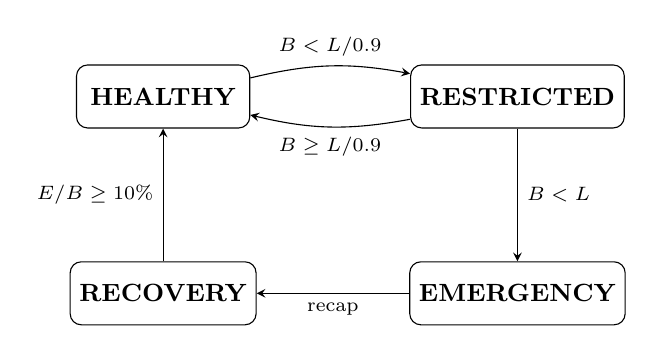
\begin{tikzpicture}[
  ->,>=stealth,
  state/.style={rectangle, draw, rounded corners, minimum width=2.2cm,
    minimum height=0.8cm, font=\small\bfseries},
  every edge/.style={draw, font=\scriptsize}
]
  \node[state] (H) at (0,0)   {HEALTHY};
  \node[state] (R) at (4.5,0) {RESTRICTED};
  \node[state] (E) at (4.5,-2.5) {EMERGENCY};
  \node[state] (V) at (0,-2.5) {RECOVERY};

  \path (H) edge[bend left=12] node[above] {$B < L/0.9$} (R);
  \path (R) edge[bend left=12] node[below] {$B \geq L/0.9$} (H);
  \path (R) edge node[right] {$B < L$} (E);
  \path (E) edge node[below] {recap} (V);
  \path (V) edge node[left] {$E/B \geq 10\%$} (H);
\end{tikzpicture}
\end{center}

% ------------------------------------------------------------
\subsection{Auto-Pause Trigger}
% ------------------------------------------------------------

\begin{equation}
  B < 0.985 \cdot L \;\Rightarrow\; \text{emergency auto-pause}
\end{equation}

This is strictly more severe than the $B < L$ emergency threshold and
triggers immediate halting of all outbound operations except burns
(which reduce $L$).

% ------------------------------------------------------------
\subsection{State Transition Events}
% ------------------------------------------------------------

Every state transition \textsc{must} emit the following event for
off-chain monitoring and audit trail:

\begin{verbatim}
event StateTransition(
    State indexed previousState,
    State indexed newState,
    uint256 backingValue,
    uint256 liabilityValue,
    uint256 equityRatio,
    uint256 timestamp,
    address triggeredBy
);
\end{verbatim}

% ============================================================
\section{Failure Behavior}
\label{sec:failures}
% ============================================================

% ------------------------------------------------------------
\subsection{MPC Halt}
% ------------------------------------------------------------

\begin{requirement}[MPC Liveness Failure]
\label{req:mpc-halt}
Two modes are defined. The protocol \textsc{must} select exactly one.

\medskip
\noindent\textbf{Mode~A: MPC required for releases.}
\begin{itemize}[nosep]
  \item Mint disabled.
  \item Release queue accumulates.
  \item No liveness guarantee until signer recovery.
\end{itemize}

\noindent\textbf{Mode~B: User-executable fallback.}
\begin{itemize}[nosep]
  \item After timeout $T$, users prove burn on source chain and
    self-relay on destination.
  \item Release executes from pre-authorized fallback path.
\end{itemize}
\end{requirement}

\begin{remark}
Mode~B is significantly stronger for institutional-grade design, even
if slower and more complex to implement.
\end{remark}

% ------------------------------------------------------------
\subsection{Stale Backing Report}
% ------------------------------------------------------------

\begin{requirement}[Backing Staleness]
\label{req:stale}
Define $\texttt{maxBackingReportAge}$ in seconds per asset.

Policy:
\begin{itemize}[nosep]
  \item If stale: \textbf{disable mint}.
  \item Allow burn and release against last confirmed backing unless
    in emergency state.
  \item Emit \texttt{BackingStale} status event.
\end{itemize}
\end{requirement}

\noindent This is the correct asymmetry: stop issuance first, preserve
exits as long as possible.

% ------------------------------------------------------------
\subsection{Strategy Loss}
% ------------------------------------------------------------

\begin{requirement}[Loss Waterfall]
\label{req:loss}
\begin{enumerate}[nosep]
  \item Realized/unrealized loss hits surplus buffer ($E$).
  \item If buffer exhausted: system enters Restricted Mint.
  \item If principal backing threatened ($B < L$): Emergency state.
  \item New deployment to strategies halted until recapitalization.
\end{enumerate}
\end{requirement}

% ------------------------------------------------------------
\subsection{Chain Reorg / Finality}
\label{sec:finality}
% ------------------------------------------------------------

\begin{requirement}[Per-Chain Finality]
\label{req:finality}
For each supported chain, define:
\begin{equation}
  \texttt{minFinalityConfirmations}[\texttt{chainId}]
\end{equation}
Mint and release \textsc{must} only occur after the finality threshold
for source events. A single global constant across all chains is
\textbf{prohibited}.
\end{requirement}

% ------------------------------------------------------------
\subsection{Oracle / Valuation Failure}
% ------------------------------------------------------------

\begin{requirement}[Oracle Failure]
\label{req:oracle}
Even for in-kind backed assets, oracle failure matters once multiple
assets exist.

Policy:
\begin{itemize}[nosep]
  \item Freeze mint for affected asset.
  \item Allow only like-for-like redemption where backing is directly
    observable.
  \item Disable cross-asset accounting based on stale prices.
\end{itemize}
\end{requirement}

% ============================================================
\section{ATS to Lux Boundary}
\label{sec:ats-boundary}
% ============================================================

\begin{requirement}[Wrapping Rule]
A security token may be transported into Lux only through a wrapper
whose compliance posture is explicitly declared and enforced at the
wrapper level.
\end{requirement}

% ------------------------------------------------------------
\subsection{Wrapper Models}
% ------------------------------------------------------------

\noindent\textbf{Strict Wrapper.}
\begin{equation*}
  \text{ATS Security} \;\to\; \text{Restricted Wrapped Security}
\end{equation*}
Properties: whitelist preserved, transfer restrictions preserved,
lockups preserved, DeFi composability limited.

Best for: institutions, lower regulatory ambiguity, near-term launches.

\medskip
\noindent\textbf{Dual Wrapper.}
\begin{align*}
  &\text{ATS Security} \;\to\; \text{Restricted Wrapper} \\
  &\text{Restricted Wrapper} \;\to\; \text{Composable Representation}
\end{align*}
Only after an explicit compliance/legal transformation. Higher product
flexibility, much more legal ambiguity.

\begin{remark}
Start strict. Dual model only after policy and counsel are settled.
\end{remark}

% ============================================================
\section{State Transition Reference}
\label{sec:transitions}
% ============================================================

\begin{table*}[t]
\centering
\caption{Allowed operations per solvency state.}
\label{tab:state-ops}
\small
\begin{tabular}{@{}lccccc@{}}
\toprule
\textbf{Operation} & \textbf{Healthy} & \textbf{Restricted} & \textbf{Emergency} & \textbf{Recovery} \\
\midrule
Mint credit               & Yes & No  & No  & No \\
Burn credit               & Yes & Yes & Yes & Yes \\
Release backing           & Yes & Yes & Policy & Yes \\
Strategy deposit          & Yes & No  & No  & No \\
Strategy withdrawal       & Optional & Accelerated & Forced & Normal \\
ATS wrapping              & Yes & Yes & No  & No \\
Backing report required   & Yes & Yes & Yes & Yes \\
\bottomrule
\end{tabular}
\end{table*}

\begin{table*}[t]
\centering
\caption{State transition conditions and authorized actors.}
\label{tab:transitions}
\small
\begin{tabular}{@{}llll@{}}
\toprule
\textbf{From} & \textbf{To} & \textbf{Condition} & \textbf{Actor} \\
\midrule
Healthy    & Restricted & $B < L / \texttt{ltvCap}$       & Automatic (on-chain) \\
Restricted & Healthy    & $B \geq L / \texttt{ltvCap}$    & Automatic (on-chain) \\
Restricted & Emergency  & $B < L$                          & Automatic (on-chain) \\
Emergency  & Recovery   & Recapitalization event           & Governance / MPC quorum \\
Recovery   & Healthy    & $E/B \geq 10\%$                  & Governance / MPC quorum \\
Any        & Emergency  & $B < 0.985 \cdot L$ (auto-pause) & Automatic (on-chain) \\
\bottomrule
\end{tabular}
\end{table*}

% ============================================================
\section{Trust Assumptions}
\label{sec:trust}
% ============================================================

\begin{enumerate}[nosep]
  \item \textbf{MPC signer set.} At least $t$-of-$n$ signers are
    honest and available for message signing. Liveness depends on
    signer availability.
  \item \textbf{Vault custody.} Strategy contracts do not have
    unilateral withdrawal authority exceeding configured risk
    parameters.
  \item \textbf{Backing oracle.} Backing attestations are delivered
    within \texttt{maxBackingReportAge} and reflect true vault state.
  \item \textbf{Chain finality.} Source chain transactions referenced
    by messages are final after
    $\texttt{minFinalityConfirmations}[\texttt{chainId}]$ blocks.
  \item \textbf{ATS compliance layer.} Security tokens wrapped into
    Lux maintain compliance posture through the wrapper contract, not
    through protocol-level enforcement.
\end{enumerate}

% ============================================================
\section{Open Questions}
\label{sec:open}
% ============================================================

Two spots require exact wording before audit:

\begin{enumerate}
  \item \textbf{Stale-backing redemptions.} Whether redemptions remain
    permissionless during stale-backing conditions, or require
    additional verification.

    \emph{Recommendation:} Stop mint, preserve exits.

  \item \textbf{Emergency undercollateralization releases.} Whether
    emergency undercollateralization pauses releases entirely or shifts
    to a queue / pro-rata / governance-controlled mode.

    \emph{Recommendation:} Stop mint, preserve claim ordering through
    an explicit emergency redemption policy (FIFO queue with
    governance-controlled release cadence).
\end{enumerate}

These are not implementation details. They are core user-rights
definitions.

% ============================================================
\section{Recommended Sequencing}
\label{sec:sequencing}
% ============================================================

\begin{enumerate}[nosep]
  \item Freeze the protocol spec (this document).
  \item Freeze the message schema (Section~\ref{sec:messages}).
  \item Freeze the solvency state machine (Section~\ref{sec:state-machine}).
  \item Map every state transition and invariant to contract checks.
  \item Deployment review and audit preparation.
\end{enumerate}

Spec first because line-by-line router review is much more valuable
once the semantics are fixed. Otherwise you end up validating code
against assumptions that are still moving.

% ============================================================
\section*{Acknowledgments}
% ============================================================

This specification incorporates review feedback from protocol
engineers, compliance counsel, and security auditors.

\bibliographystyle{plain}
\bibliography{references}

\end{document}
